\section{Subject}
\begin{figure}[htb!]
\centerline{
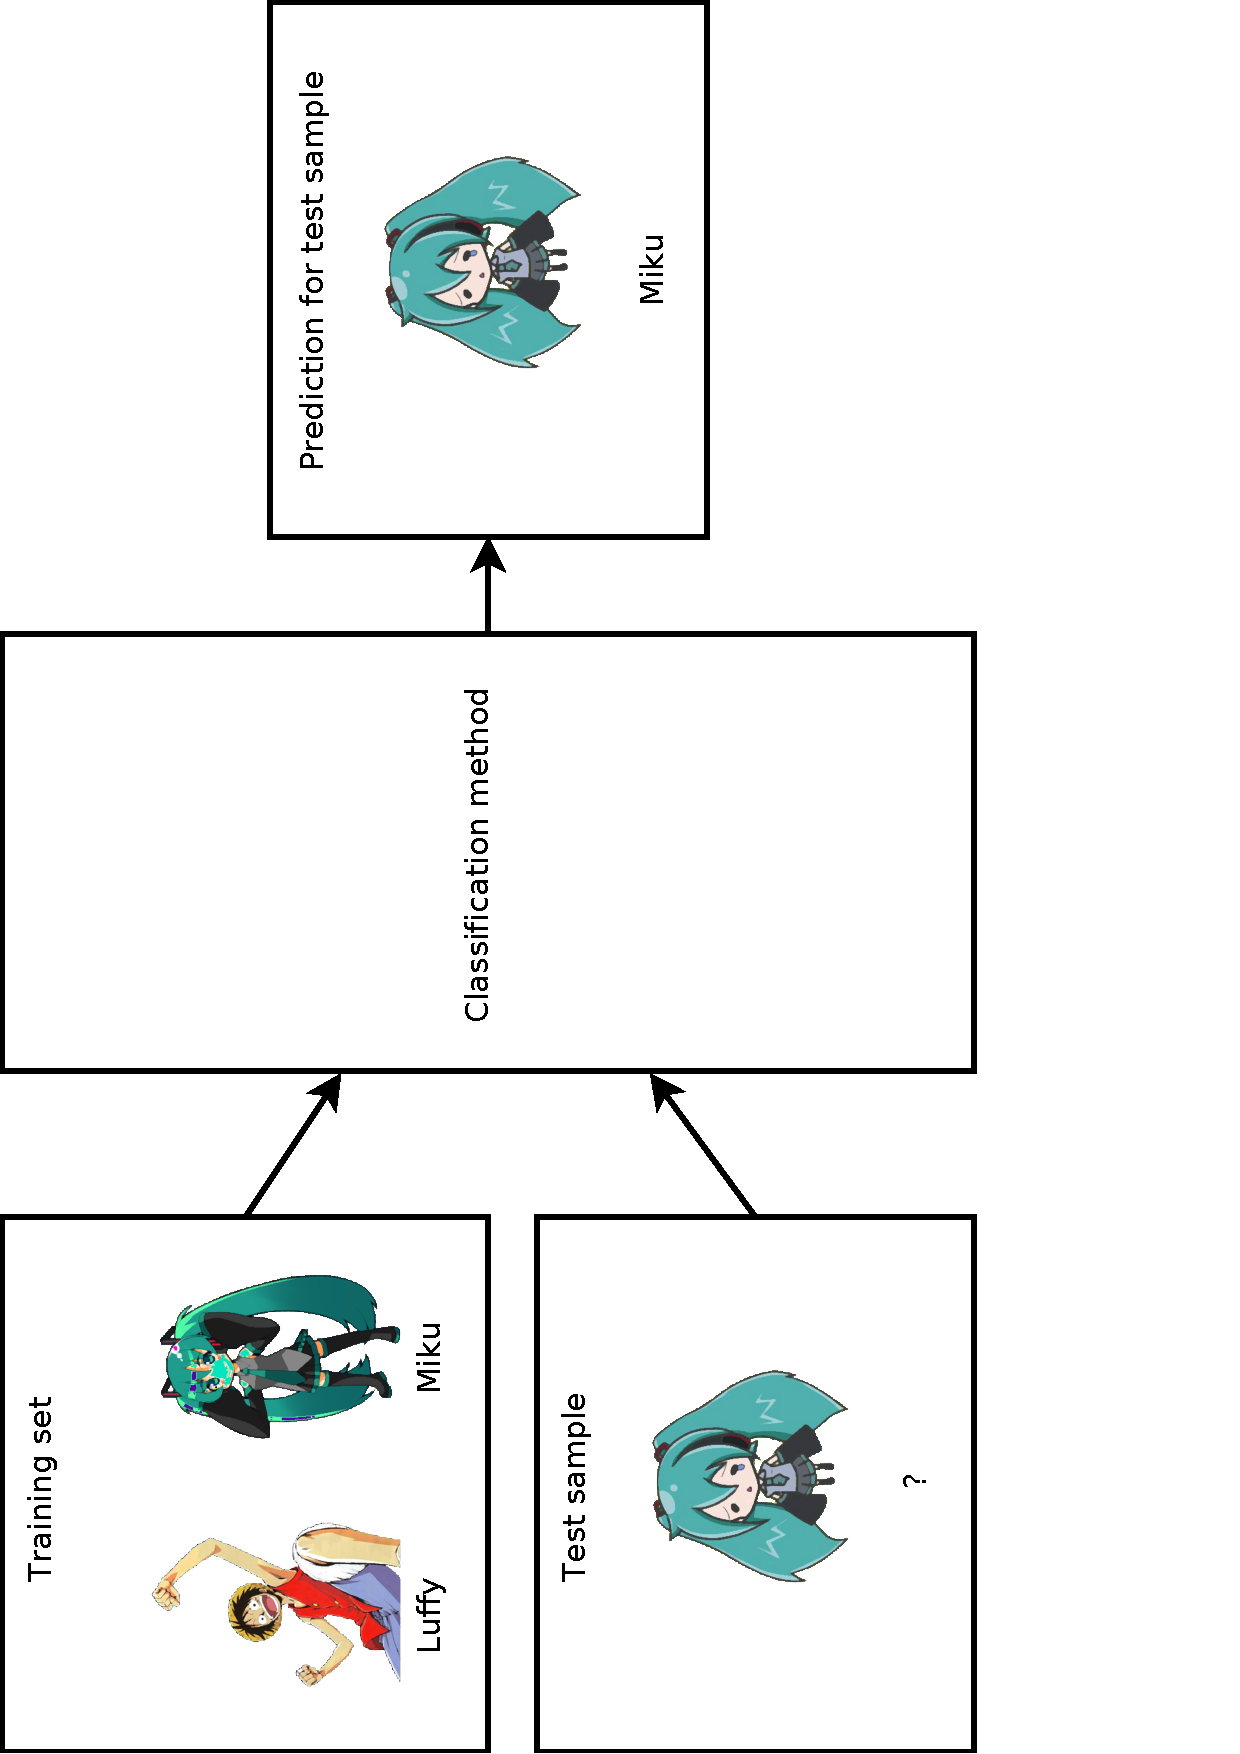
\includegraphics[height=1.2\textwidth, angle=270,clip=true,trim=0 0 4cm 0]{images/trainingPredictionDiagram.pdf}
}
\caption{Diagram depicting how training and prediction work for the method.}
\label{fig:trainingPredictionDiagram}
\end{figure}

The subject of my work here was to design a computer algorithm able to automatically identify characters from color images. It should take the shape of a supervised or semi-supervised classification method, meaning it should be able to identify an image by comparing it against a training set. Said training set may consist of labeled images - images which are known to depict a certain character - as well as unlabeled images in the case of semi-supervised classification (\autoref{fig:trainingPredictionDiagram}).

\section{Position in the laboratory}
I worked in the Sakamoto laboratory as a research student.
\section{Previous studies}
Previous work in the laboratory by graduate student Yuki Nakagawa on the animation character identification problem identified a segmentation method\cite{felzenszwalb2004efficient} and a classification method\cite{harchaoui2007image} for the problem. A dataset of animation character images was also previously constituted in the laboratory.

There is little previous literature on animation character image analysis, and all of it is in Japanese. There has been work on identifying artist information from images in \cite{itamochi2012identification}, whose abstract has been translated to me by professor Sakamoto.

\section{Objectives}

\begin{figure}[htb!]
\centering
\begin{subfigure}{.3\textwidth}
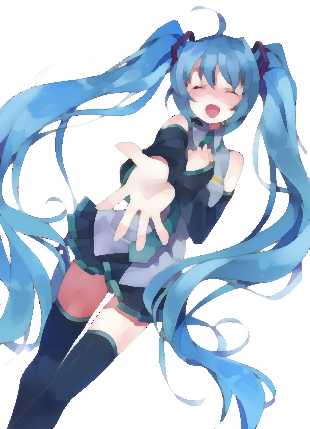
\includegraphics[width=\textwidth]{images/miku_e.png}
\end{subfigure}
\begin{subfigure}{.3\textwidth}

\includegraphics[width=\textwidth]{images/miku_c.png}
\end{subfigure}
\begin{subfigure}{.3\textwidth}

\includegraphics[width=\textwidth]{images/miku_d.png}
\end{subfigure}
\caption{Images for one character illustrating differences in posture, exaggerations, occlusion and artist differences.}
\label{fig:animationImagesVariations}
\end{figure}

The first objective was to design a method which would improve on the state of the art in animation character identification, in terms of recognition rate, clustering quality or run time performance. The envisioned application domain being automatic image annotation for web artist communities such as Pixiv or deviantArt, it should also be able to handle large datasets.

A secondary objective was to improve on the state of the art in the fields of computer vision and machine learning through the challenges specific to animation characters. There is for instance a large literature on human face recognition \cite{turk1991eigenfaces} \cite{belhumeur1997eigenfaces}, but such methods fail to account for meaningful color information in animation images as well as variations introduced by character posture, exaggerations, occlusion of body parts and differences between artists (\autoref{fig:animationImagesVariations}). Many classification and clustering methods also require data to form convex clusters (for instance $k$-means clustering), which is rarely the case with animation images because of previously mentioned variations, so recent research involving non-linear embeddings of data were of particular interest \cite{roweis2000nonlinear} \cite{belkin2003laplacian} .

\section{Planning}
No provisional planning was established upon my arrival. The only milestones were:
\begin{itemize}
\item Deadline for paper submission to the JCEEE Kyushu 2013 conference \cite{jceeeKyushuWebsite} at the end of August.
\item Paper presentation at the the JCEEE Kyushu 2013 international sessions on the $24^{th}$ of September in Kumamoto.
\end{itemize}